\documentclass[11pt]{scrartcl}
\usepackage{tkz-graph}


\begin{document}
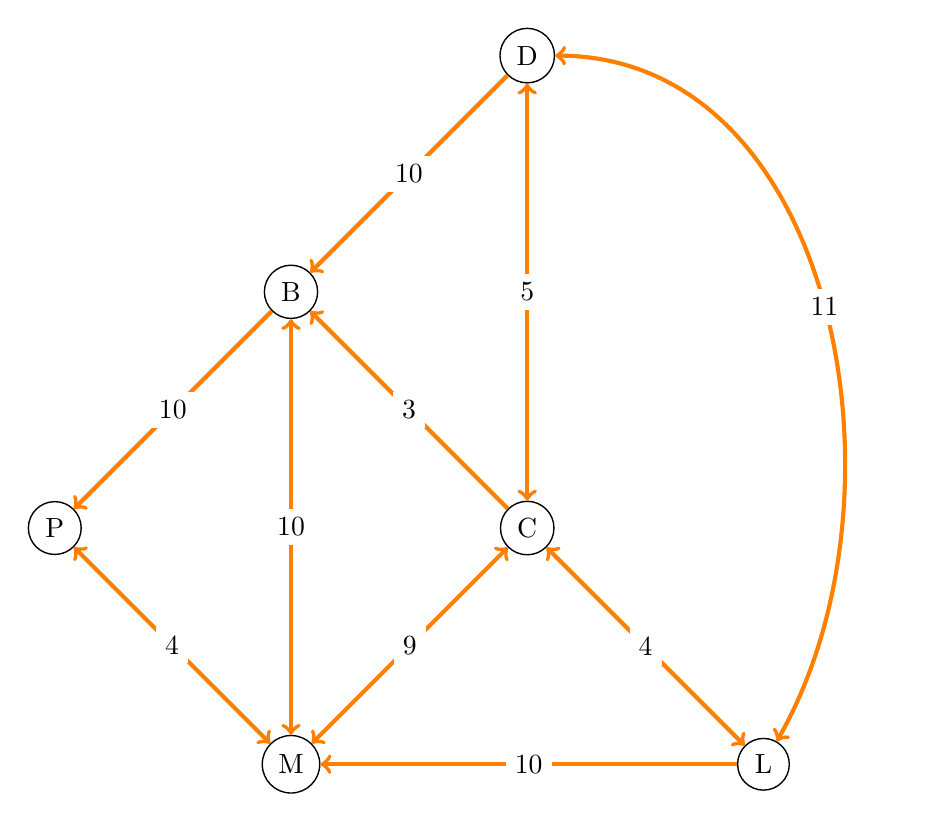
\begin{tikzpicture}
 \SetUpEdge[lw         = 1.5pt,
            color      = orange,
            labelcolor = white]
  \GraphInit[vstyle=Normal] 
  \SetGraphUnit{3}
  \tikzset{VertexStyle/.append  style={fill}}
  \Vertex{P}
  \NOEA(P){B}  \SOEA(P){M} \NOEA(B){D}
  \SOEA(B){C}  \SOEA(C){L}
  \tikzset{EdgeStyle/.style={->}}
  \Edge[label=$3$](C)(B)
  \Edge[label=$10$](D)(B)
  \Edge[label=$10$](L)(M)
  \Edge[label=$10$](B)(P)
  \tikzset{EdgeStyle/.style={<->}}
  \Edge[label=$4$](P)(M)
  \Edge[label=$9$](C)(M)
  \Edge[label=$4$](C)(L)
  \Edge[label=$5$](C)(D)
  \Edge[label=$10$](B)(M)
  \tikzset{EdgeStyle/.style={<->,relative=false,in=0,out=60}}
  \Edge[label=$11$](L)(D)
\end{tikzpicture}
\end{document}
